\documentclass[10pt,english]{article}
\usepackage[utf8]{inputenc}
\markright{Weedop \hfill}
\usepackage{geometry}
\usepackage[labelfont=bf]{caption}
\usepackage{makecell}
\geometry{verbose,letterpaper,tmargin=2.54cm,bmargin=2.54cm,lmargin=2.54cm,rmargin=2.54cm}
%\geometry{verbose,letterpaper,tmargin=.1cm,bmargin=.1cm,lmargin=.1cm,rmargin=.1cm}
\usepackage{graphicx}
\DeclareGraphicsExtensions{.pdf,.png}
\usepackage{amssymb,amsmath}
\usepackage{epstopdf}
\usepackage{tocbibind}
\usepackage[toc,page]{appendix}
\usepackage{supertabular}
\DeclareGraphicsRule{.tif}{png}{.png}{`convert #1 `dirname #1`/`basename #1 .tif`.png}
\usepackage{url}
\usepackage{subcaption}
\usepackage{caption}
\usepackage[super]{nth}
\usepackage{lineno} \linenumbers
\usepackage[doublespacing]{setspace}
\usepackage[parfill]{parskip}
\setlength{\parindent}{0pt}
\usepackage{csquotes}
\usepackage[backend=biber,
  natbib=true,
  style=authoryear,
  citetracker=true,
  maxcitenames=2,
  uniquelist=false,
  uniquename=false]{biblatex}

\AtEveryCitekey{\ifciteseen{}{\defcounter{maxnames}{2}}}
\renewbibmacro{in:}{}
\DeclareFieldFormat[article, inbook, incollection, inproceedings, misc, thesis, unpublished]{title}{#1}
\DeclareFieldFormat[article, inbook, incollection, inproceedings, misc, thesis, unpublished]{pages}{#1}
\addbibresource{rotation-project_bahl-lab_high-path-h5-egypt_avian-human.bib}

\DeclareFieldFormat[article]{volume}{#1}
\setlength{\bibhang}{0pt}

\usepackage{changes}
\setdeletedmarkup{\textcolor{red}{\sout{#1}}}

\begin{document}
\setlength{\parindent}{0pt}

\section*{Title page}

\textbf{Article title}: Exploration of Interhost Transmission of Highly Pathogenic H5N1 Influenza in Egypt

\textbf{Authors:} K.\ Bodie Weedop$^{1*}$

$^1$ Integrated Life Sciences, Franklin College of Arts and Sciences, University of Georgia, Athens, GA, 30602, USA

$^*$To whom correspondence should be addressed: K.\ Bodie Weedop (\url{kbweedop@gmail.com})

\clearpage

\section*{Introduction}
Highly pathogenic Avian influenza virus (HPAIV) H5N1 has become particularly concerning in countries throughout Eastern Asia, Southeast Asia and Africa. HPAIV H5N1 was orginally detected in geese in 1996 and then quickly spread to humans without any intermediate ``mixing vessel'' \autocite{Claas1998, Chen2005}. After an outbreak in Hong Kong in 1997, HPAIV H5N1 has spread, in spite of countermeasures, to a variety of different avian (wild and domesticated) and mammal hosts \autocite{Chan2002, Kaplan2013}. Additionally, the virus quickly spread geographically via wild migratory avian hosts to be detected in European, Middle Eastern and African countries \autocite{Alexander2007, Salzberg2007}. In 2006, a national surveillance program in Egypt detected cases of HPAIV H5N1 in backyard poultry and later determined the spread originated from wild migratory birds \autocite{Saad2007, Abdelwhab2015}. Since this initial detection, Egypt has been declared as an HPAIV H5N1 endemic country \autocite{International2007}. However, with many control measures and vaccine efforts having failed to stifle further spread of HPAIV H5N1, Egypt is being monitored closely as a potential hotspot for an influenza pandemic \autocite{Kayali2011, Kayali2016, Young2018}. 

HPAIV H5N1 has spread across, and since circulated in, populations of both wild migratory fowl and domesticated birds in Egypt \autocite{Kayali2014}. Since HPAIV H5N1 became enzootic in Egypt, antigenic diversity has increased due both antigenic drift and vaccine pressure leading to cocirculating endemic lineages in the domesticated bird population (clades 2.2.1, 2.2.1.1, 2.2.1.2) \autocite{Who2012, Kayali2014, Smith2015}. This broad spread, circulation of lineages, and increased diversity may be due to frequent contact between wild and domesticated birds as well as rearing of multiple domesticated bird species such as chickens, ducks, geese and turkeys in commercial and barkyard farms. Infections in the commercial sector and backyards play an important role in H5N1 epidemiology in both avian and human hosts. The commercial sector has been reported to be a likely resevoir of HPAIV H5N1 lineages \autocite{Kayali2011}. Where, in contrast, backyard poultry are under little to no biosecurity measures and have been described as the main source for bird to human transfer \autocite{Kandeel2010}. Transfer of HPAIV H5N1 between commercial and backyard birds has been driven by a number of factors including legal and illegal bird trade (live bird markets), commercial employees, and used commercial equipment \autocite{Abdelwhab2015}. As infection of both commercial and backyard avian hosts continues, further antigenic drift and recombination of HPAIV H5N1 with cocirculating avian influenza virus (AIV) subtypes (H5N8 and H9N2) are a major concern when considering the possibility of a pandemic \autocite{Neumann2012}.

While HPAIV H5N1 has had devastating effects on Egyptian domesticated poultry populations, Egypt is also one of few countries that has seen large numbers of human infection of HPAIV H5N1. World Health Organization (WHO) data on confirmed cases of human infection and deaths attributed to HPAIV H5N1 have occurred in Egypt and Indonesia \autocite{Who2019}. While having more confirmed cases of the virus than any other country, the fatality rate in Egypt (\textasciitilde 33\%) is lower compared to the global fatality rate (\textasciitilde 53\%). This may be due to most lineages of H5N1 in Egypt are susceptible to the NA-inhibitor, oseltamivir \autocite{Kayali2011}. Interestingly, transmission to human hosts has been seen disproportionately in women and children \autocite{Fasina2010, Abdelwhab2011}. This phenomena has been attributed to women and children having increased exposure (i.e.\ playing, de-feathering, slaughter) to backyard poultry. While there have been many cases of human infection in Egypt, human-to-human transmission of HPAIV H5N1 has been shown to be inefficient \autocite{Schroedl2010}. The limited number of human-to-human transmissions that have been reported in Egypt and other afflicted countries are typically clustered in households \autocite{Ungchusak2005, Kandeel2010, Gomaa2014}. As human infection of HPAIV H5N1 continues via infected avian hosts or human-to-human transmission, there is increased opportunity for antigenic drift and immune selection, antiviral resistance, and/or recombination with other circulating AIVs. Such events could allow for HPAIV H5N1 to infect humans more efficiently and/or recombine to ultimately form a pandemic strain infecting humans.

HPAIV H5N1 in Egypt provides a valuable system to investigate evolutionary and epidemiological dynamics of a highly pathogenic endemic strain of AIV. Understanding the diversification of the virus in the population as well as patterns of infection in humans will help guide biosecurity measures, culling procedures, and education for the general public. In this investigation, I show a preliminary, exploratory analysis of HPAIV H5N1 antigenic evolution while considering infection of avian and human hosts. This analysis is exploratory in nature and done for educational purposes. 

\section*{Methods}

\subsection*{Sequence data collection and alignment}

In order to explore interhost transmission of HPAIV H5N1, I collected full length hemagglutinin (HA) sequences from cases of HPAIV H5N1 in both humans and avian hosts from 2006 to 2017 from the Influenza Virus Sequence Database maintained by the National Center for Biotechnology Information (NCBI). Metadata for all samples included a geographical location (at least country of origin), type of host, and date the sample was taken. Some sequences did not have the complete date (YYYY/MM/DD) the sample was taken and only included the year or month and year. Metadata with only the year (2011) or year and month (2011/03) were imputed with the first day of the month of June (2011/06/01) or the first day of the month given in the metadata (2011/03/01), respectively. Duplicate sequences were removed from the analysis. For the purposes of this preliminary analysis, I performed random subsampling to select 200 sequences. This was primarily done to reduce the amount of sequences for the final analysis and, therefore, reduce computational time to completion of the Bayesian Mixed Chain Monte Carlo (BMCMC) analysis. A final 167 full-length HA sequences were then aligned using MAFFT and alignment trimming was performed manually after alignment using BioEdit \autocite{Katoh2013, Hall1999}.

\subsection*{Phylogenetic analysis}

In order to explore and provide an initial estimate of phylogenetic and temporal signals, I applied maximum likelihood approach on an initial tree using RAxML (v8.2.12) and tempEST (v1.5.3) \autocite{Stamatakis2014, Rambaut2016}. I used the BMCMC approach as implemented by BEAST v1.10.1 to provide temporal phylogenies \autocite{Drummond2007}. I used the generalized time reversal (GTR) substitution model while allowing rate heterogeneity using invariable sites (I) and a discrete (4 rate categories) gamma distribution ($\gamma$). Additionally, I used an uncorrelated relaxed clock model to infer the evolutionary time scale of the alignment sequences. For the tree prior, I used a smooth Gaussian process prior which assumes population size changes evenly over time with the GMRF Bayesian Skyride tree prior as provided by BEAST (v1.10.1) \autocite{Drummond2007, Minin2008}. I performed six separate runs of the BMCMC sampling using chain length of 100 million with a 10\% burn-in removed. The six independent runs were compared to ensure statistical support in the effective sample size values (ESS) and adequate sampling. I used a posterior probability limit of 95\% on 9000 trees to produce a maximum clade credibility consensus tree using the software packages LogCombiner (v1.10.1) and TreeAnnotator (v1.10.1) \autocite{Drummond2007}.

\section*{Results}

Five out of the six independent BEAST analyses showed significant statistical support with all ESS values being greater than 200. The single BEAST run that did not converge during the BMCMC analysis was discarded and not included in the consensus tree. Many of the nodes are well supported in the final temporal phylogeny show high posterior probability values ($>$0.95; Fig. \ref{gene-tree}).

A reconstruction of the effective population size and characterization of HPAIV H5N1 population dynamics seen from when the virus was first introduced to Egypt to 2017 (Fig. \ref{gmrf-plot}). The estimation of Egyptian HPAIV H5N1 population size dynamics shows a significant, and expected, increase over earlier years (2006-2008). In more recent years, the effective population size shows a cyclical trend with no obvious increase.

\subsection*{Seasonal aspects of H5N1 HPAIV infection}

It is not clear that there are year round occurrence of human infection (Fig. \ref{gene-tree}). The results here suggest that human cases are occurring in cycles during the winter/spring season. However, subsampling the data removed a number of sequences from human infection which is likely the cause of not seeing data consistent with previous research. 

\subsection*{Clustering of human infection}

Cases of human infection are clustered together by relatedness rather than spread randomly throughout the tree. This can be seen in the relatively large numbers of human cases during the winter/spring months in 2009 and 2010, respectively (Fig. \ref{gene-tree}). This same phenomena is seen again during the same season of 2014 and 2015. No data is provided with sequences to show whether hosts were located in the same household. Clades where human cases are clustered in the phylogeny show posterior support. 

\clearpage
\begin{figure}[!ht]
  \center
  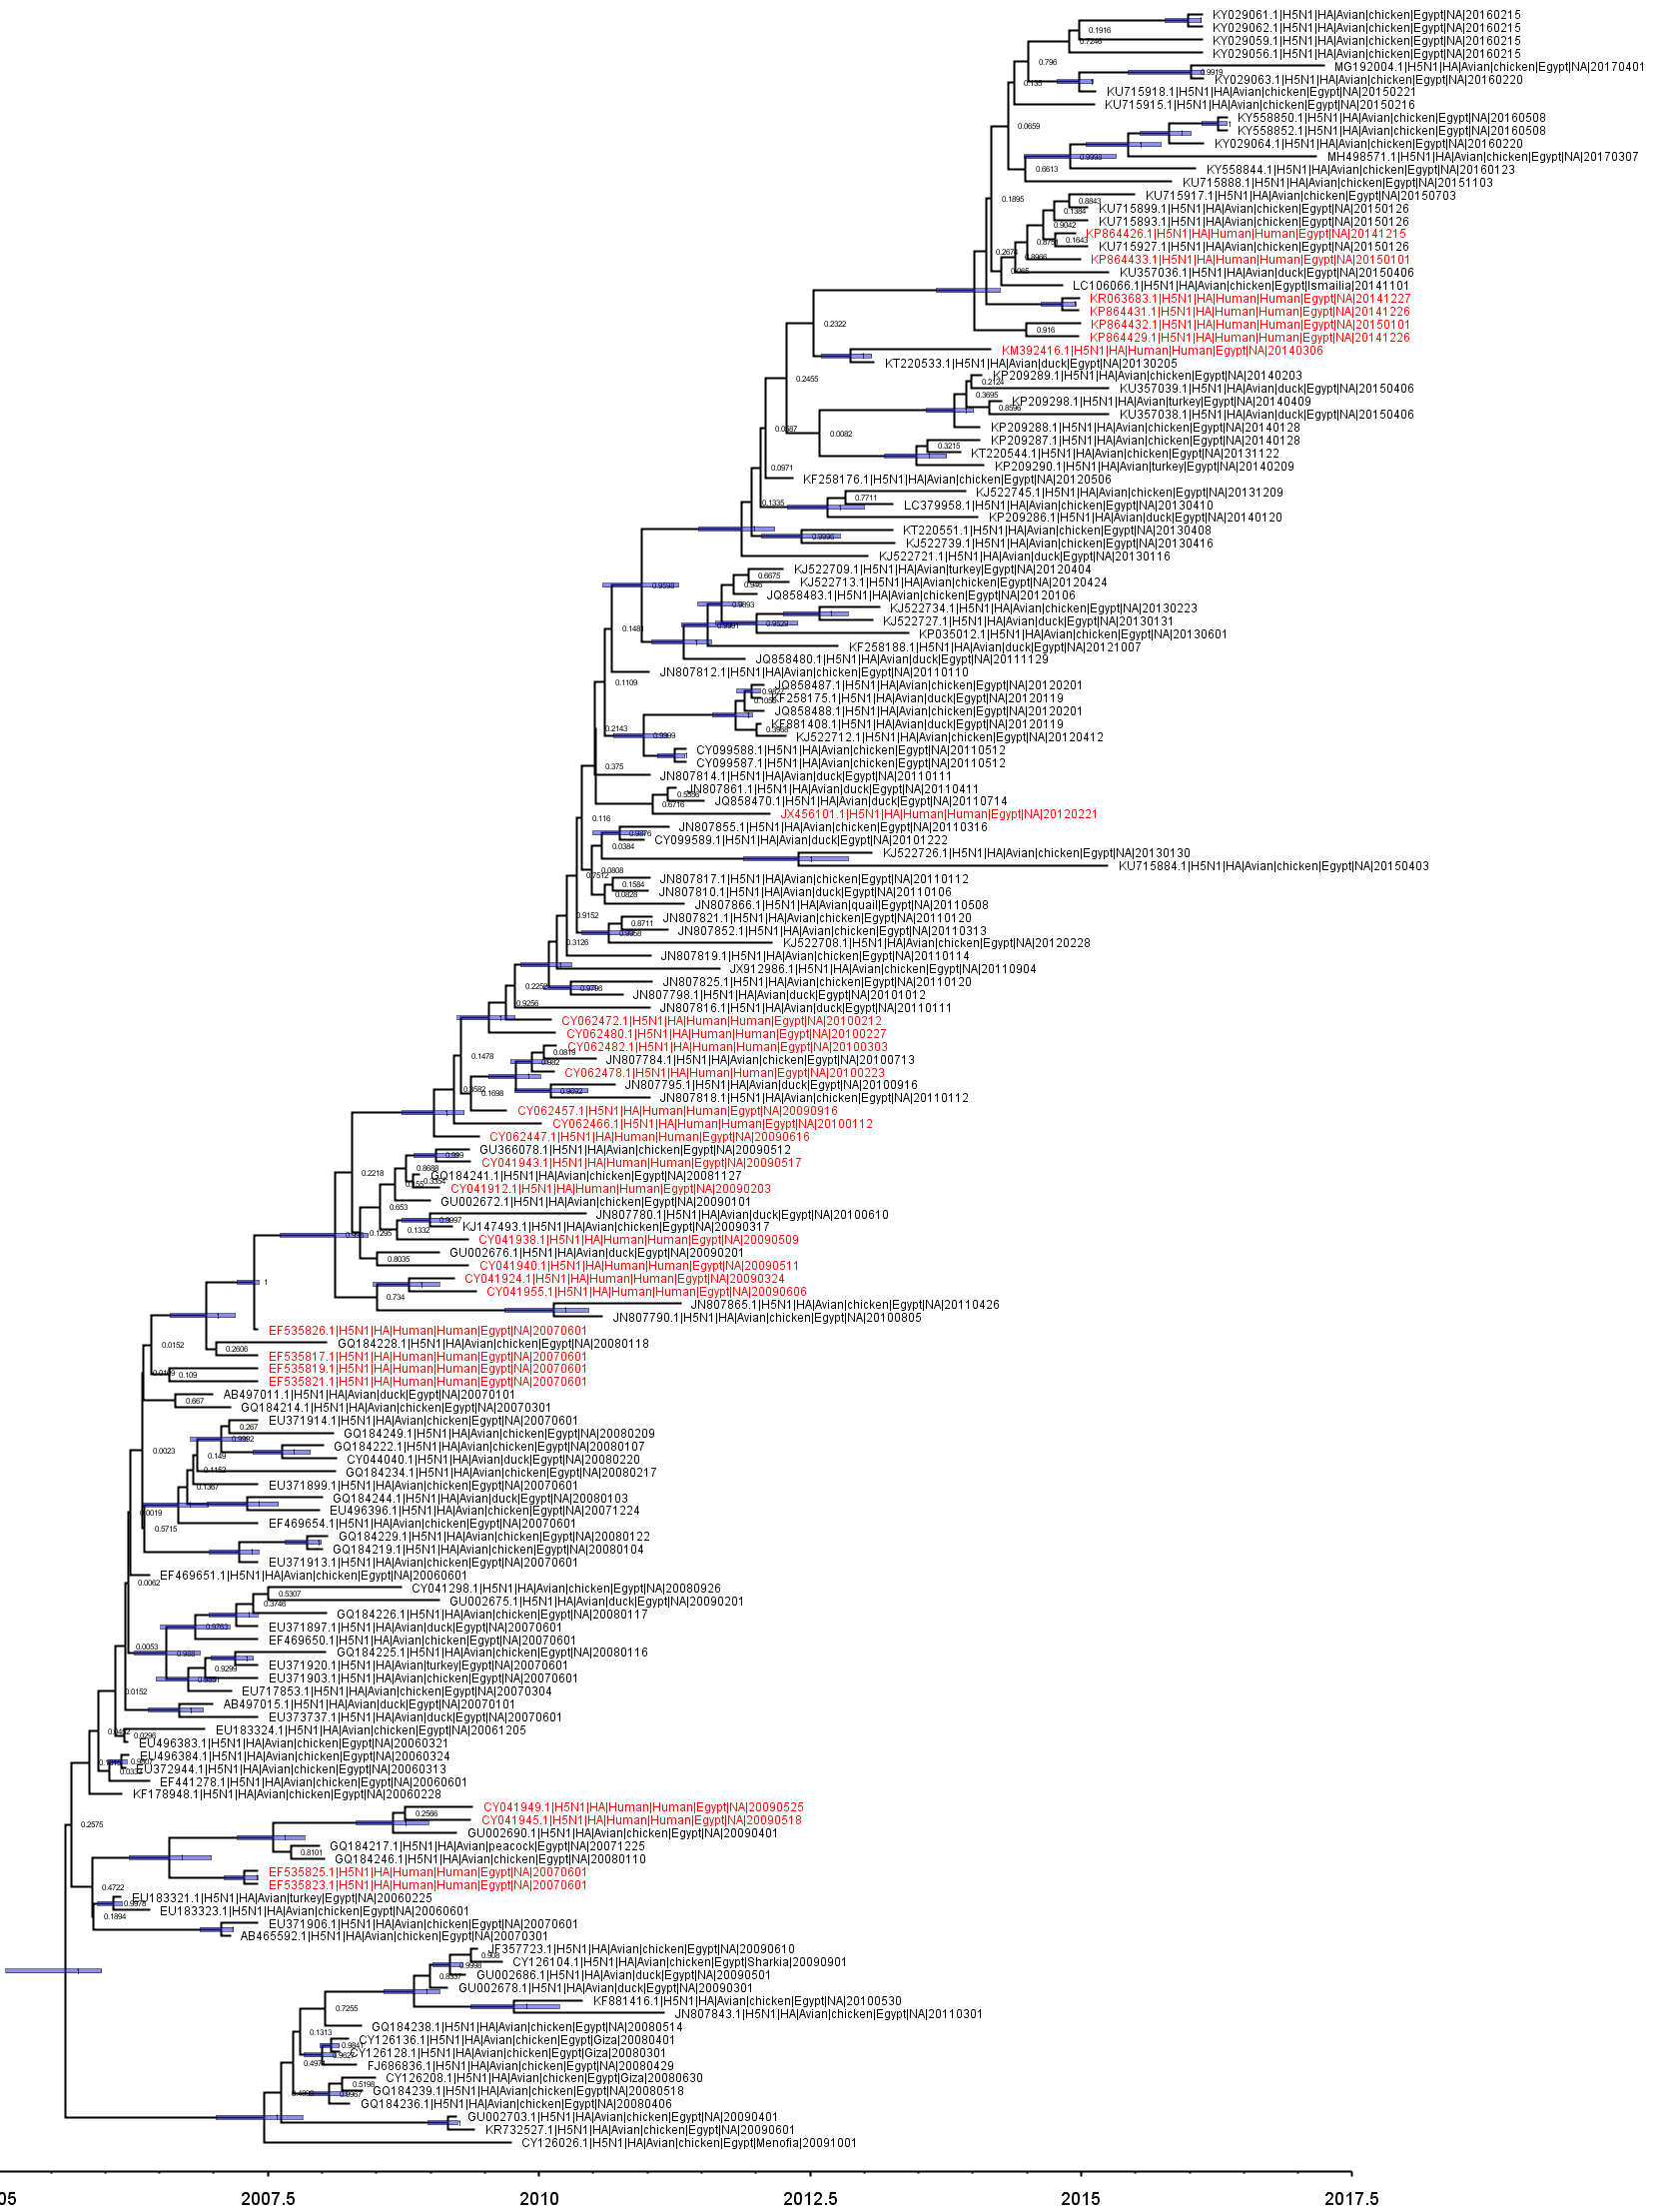
\includegraphics[width=.75\textwidth]{./figures/annotated_combined.png}
  \caption{\textbf{Phylogenetic tree of HA gene sequences from cases of avian and human infection of HPAIV H5N1.} Phylogenetic analysis was done using BMCMC method as performed by BEAST v1.10.1. Nodes are labeled with their posterior probability combined with a bar demonstrating the 95\% highest probability density (HPD) interval. All sequences from human infection have labels highlighted in red.}
  \label{gene-tree}
\end{figure}
\clearpage

\clearpage
\begin{figure}[!ht]
  \center
  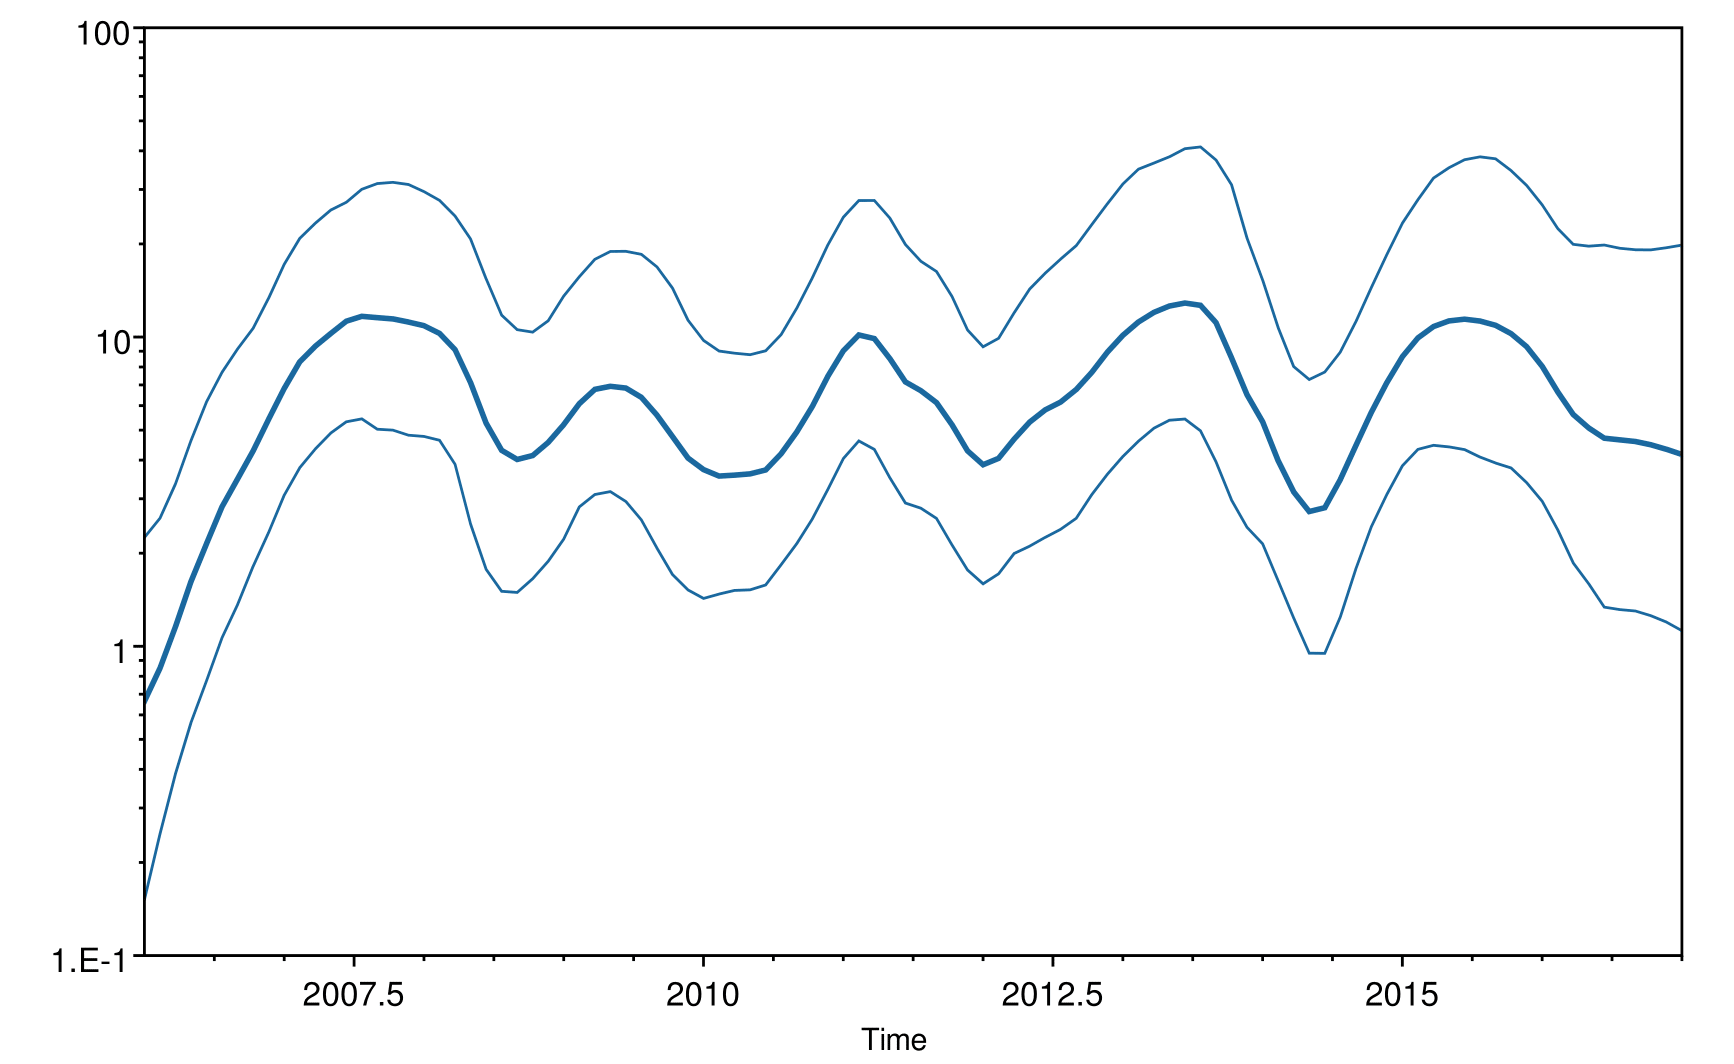
\includegraphics[width=.75\textwidth]{./figures/gmrf-plot.png}
  \caption{\textbf{Gaussian Markov Random Field (GMRF) Bayesian Skyride plot showing the reconstruction of HPAIV H5N1 demographic history.} The plot demonstrates the relationship between the log effective population size and time. The dark blue line represents the median estimate of effective population size while the lighter blue boundary lines demonstrate the boundaries of the 95\% HPD.}
  \label{gmrf-plot}
\end{figure}
\clearpage

\section*{Discussion}

I performed this analysis to explore different phylogenetic, evolutionary, and epidemiological aspects of HPAIV H5N1 while considering cases of infection in both avian and human hosts. This analysis is preliminary and, as the results suggest, an increased sample size is needed to make conclusions on the nature of interhost transmission of HPAIV H5N1. However, this preliminary analysis does support previous research showing that human-to-human transmission of HPAIV H5N1 is sporadic and with no further diversification (Fig. \ref{gene-tree}). I present results in this analysis that show clustering of human cases of H5N1 temporally and phylogenetically. However, it is difficult to know the nature of this clustering without increased numbers of sequences. Also, additional metadata such as relationships between hosts or location data is needed to make further conclusions. Low resolution of data and the lack of metadata does not allow for any further conclusions.

While having additional, detailed data will help increase the resolition of our analysis, there are a number of alternative questions concerning the dynamics of HPAIV H5N1 in Egypt. In the future, investigating transmission, and subsequent evolutionary events, of HPAIV H5N1 and other influenza subtypes in Egyptian swine and other mammal host populations will provide insight on potential recombinant influenza viruses. There has been some surveillance on this front to show that multiple AIVs and human influenza viruses are present in Egyptian swine \autocite{Gomaa2018}.

While this is a preliminary analysis, I think that it provides an example of exploring aspects of interhost transmission of HPAIV H5N1. Complexity of such an analysis is reduced given that most infections in Egypt are from established and circulating lineages. Molecular surveillance of HPAIV H5N1 while considering avian and human populations could provide information on further diversification of the virus isolate to human hosts. Such information may alert biosecurity officials that the virus is increasing specificity to human hosts. 

\section*{Acknowledgments}

I would like to thank everyone at the Bahl Lab. Justin provided me the opportunity to carry out this analysis, gain familiarity with his phylodynamics pipeline and learn from his lab members. Lambodhar (Lambo) was incredibly helpful and walked me through some of the murky waters. Jiani directed me toward valuable literature that helped inform my analysis.  

\clearpage
\printbibliography

\end{document}
%%% Local Variables:
%%% mode: latex
%%% TeX-master: t
%%% End:
